\section{Training versus Testing} % (fold)
\noindent
{\color{LightRubineRed} \rule{\linewidth}{1mm} }
\begin{bclogo}{Importance}
\begin{align*}
\mathbb{E}_{out}(g) \underbrace{\approx}_{\text{test}} \mathbb{E}_{in}(g) \underbrace{\approx}_{\text{train}} 0
\end{align*}
\end{bclogo}
\subsection{Effective Number lines} % (fold)
\label{sub:effective_number_lines}
\begin{center}
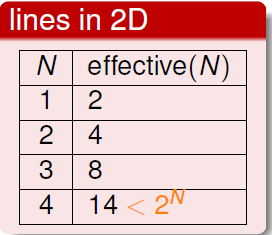
\includegraphics[width=6cm, height=6.5cm]{lecture5_2}\\
\end{center}
\begin{itemize}
	\item effective(N) can replace $M$ and
	\item effective(N) << $2^N$
\end{itemize}
\subsection{Effective Number of Hypotheses}
dichotomies 二分 \par
\begin{center}
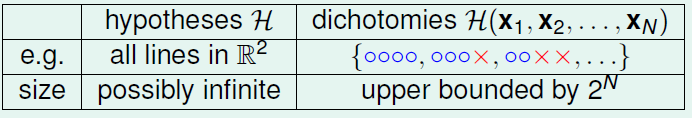
\includegraphics[width=10cm, height=4cm]{lecture5_1}\\
\end{center}
\begin{align*}
m_{\mathcal{H}}(N)=2^N \rightleftharpoons 
\end{align*}
text{exists} $N$ \text{inputs that can be shattered}

\subsection{Break Point}
if no $K$ inputs can be shatted by $H$, \par
call k a break point for $H$。
\begin{align}
m_{\mathcal{H}}(k) < 2^K \\
k+1,k+2,.. \text{also break points} \\
\end{align}
break points跟成长函数是有关的 。 \\

\begin{center}
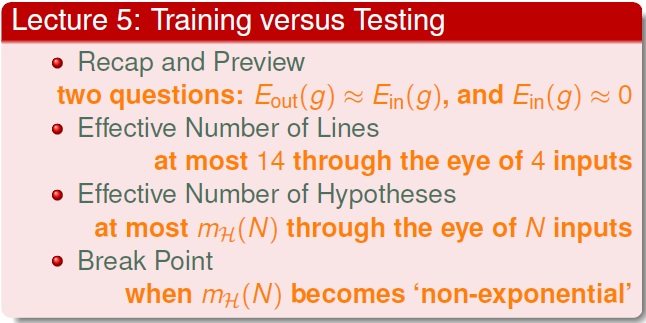
\includegraphics[width=10cm, height=6cm]{lecture5_sum}\\
\end{center}
% subsubsection effective_number_lines (end)
% section section_name (end)
\noindent
{\color{RubineRed} \rule{\linewidth}{1mm} }